\documentclass[11pt]{article}

% -------------------------------------------------------------------------------- %

% *** LANGUAGE ***
%\usepackage[italian]{babel}
%\usepackage[applemac]{inputenc}

% *** PAGE LAYOUT ***
\usepackage{geometry}     
%\geometry{a4paper}                   
%\geometry{landscape}                % Activate for for rotated page geometry
%\usepackage[parfill]{parskip}       % Activate to begin paragraphs with an empty line rather than an indent

\geometry{a4paper,tmargin=2cm,bmargin=2cm,lmargin=2.5cm,rmargin=2.5cm}

% *** DEFAULT FONT SELECTION ***
\usepackage[T1]{fontenc}
\usepackage{lmodern}
\renewcommand*\familydefault{\sfdefault} %	Only if the base font of the document is to be sans serif

% *** IMAGES ***
\usepackage{graphicx}
\usepackage{subfig}


\title{
	{\Large Laboratory report 0: PID Design and Estimation Parameters \\
	 \large Group 2, Tuesday Shift}
}
\author{Baron Davide, Bonetto Alessio, Mustacchi Marco, Piron Luca Vittorio}
\date{March 22, 2022}


\begin{document}

\maketitle

\section{Introduction}

	\subsection{Activity Goal}
	The goal of this laboratory activity is to design a position PID controller for a DC servomotor and to estimate the values
	of viscous friction $\tau_{sf}$, static friction $B_{eq}$ and the inertial torque $J_{eq}$. \\
	For the PID design, the Bode's method (explained in Sec. 3.2 of Handout 0) has been used, in order to achieve the following performance specifications:
	
	\begin{itemize}
		\item perfect steady state tracking of step position (load side) reference
		\item perfect steady state rejection of constant torque disturbances
		\item step response (at load side) with settling time $t_{s,5\%} \le 0.15s$ and overshoot $M_{p} \le 10\%$
	\end{itemize}

	\subsection{Model used}
	The black box $\textit{Quanser\_SRV02\_block}$ has been used in order to replace the DC motors physically present in the laboratory
	and faithfully reproduce the behaviour of the real one.

\section{Design of PID-controller}
The continous time transfer function of the controller $C(s)$ is:
	\begin{equation}
		C(s) = K_P +\frac{K_I}{s} + K_D\frac{s}{1 + sT_L}
	\end{equation}
with a real derivative action $\frac{s}{1 + sT_L}$ instead of ideal derivative (since the last one is not physically implementable). \\
For the synthesis of the controller, the Bode's mehod has been used, which leads to the following values:

	\begin{equation}
		K_P = 8.91 \quad K_I = 81.64 \quad K_D = 0.1218 \quad T_L = 0.0059s
	\end{equation} 
However, these parameters need to be adjusted "manually" in order to reach all the required performance specifications. The modified parameters are:
	\begin{equation}
		K_P = 11 \quad K_I = 40 \quad K_D = 0.125 \quad T_L = 0.0059s
	\end{equation}

These values have been used in order to control the DC motors dynamics and later, to estimate the frictions parameters and the inertial
torque parameter.

\newpage
\section{Estimation of Parameters}
	\subsection{Viscous and static friction}
	For the evaluation of static and viscous friction the procedure explained in Sec 4.1 of Handout 0 has been used. The result of the calculations provide:
		\begin{equation}
			\hat B_{eq} = 1.25\cdot10^{-6}Nm/(rad/s) \quad \hat\tau_{sf} = 0.0057Nm
		\end{equation}

		\begin{figure}[h!]
		\centering
		\subfloat[]{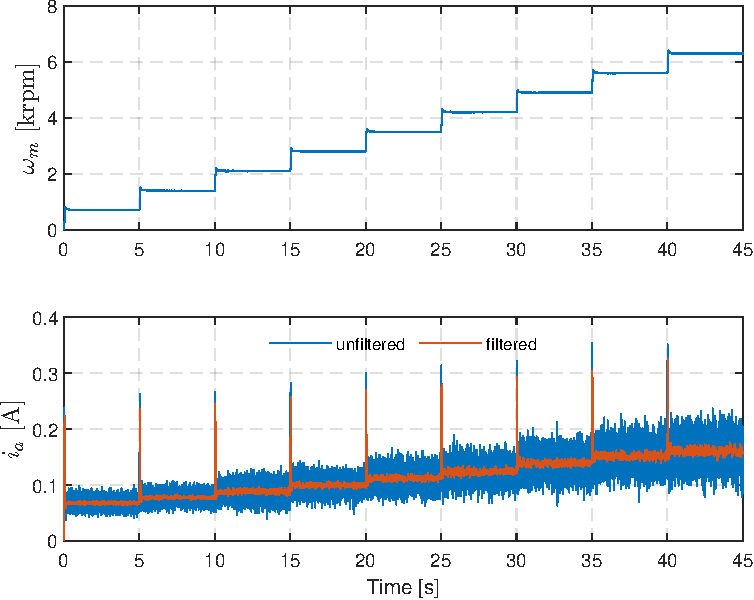
\includegraphics[scale=0.60]{images/Friction_Estimates_ia_wm_Plot}}\quad
		\subfloat[]{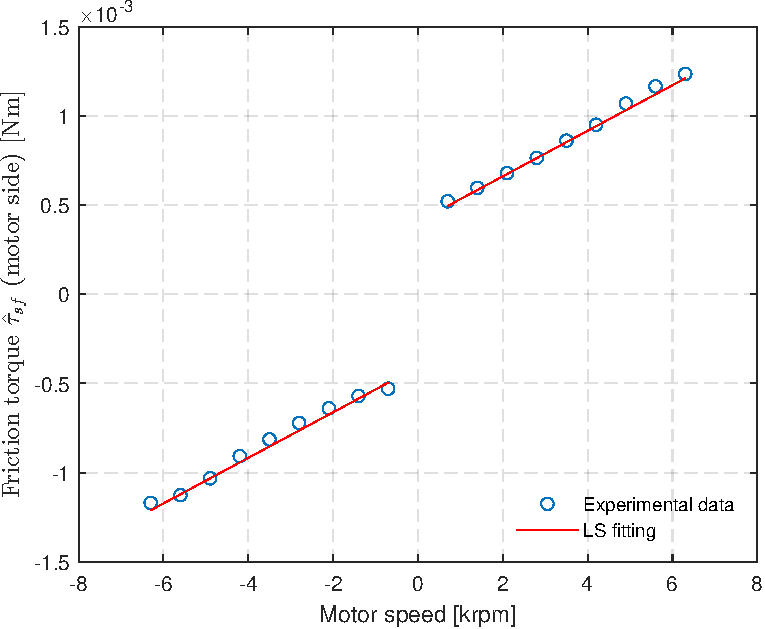
\includegraphics[scale=0.60]{images/Friction_Estimates_tau_Plot}}
		\caption{Friction estimation test: (a) experimental data (for positive speed profile); (b) LS estimation of friction parameters.}
		\end{figure}

	\subsection{Inertial torque}
	For the evaluation of inertial torque component, the procedure explained in Sec 4.2 of Handout 0 has been used. The result of the calculations provide:
	\begin{equation}
		\hat J_{eq} = 5.63\cdot10^{-7}Kg\cdot m^2
	\end{equation}

		\begin{figure}[h!]
		\centering
		\subfloat[]{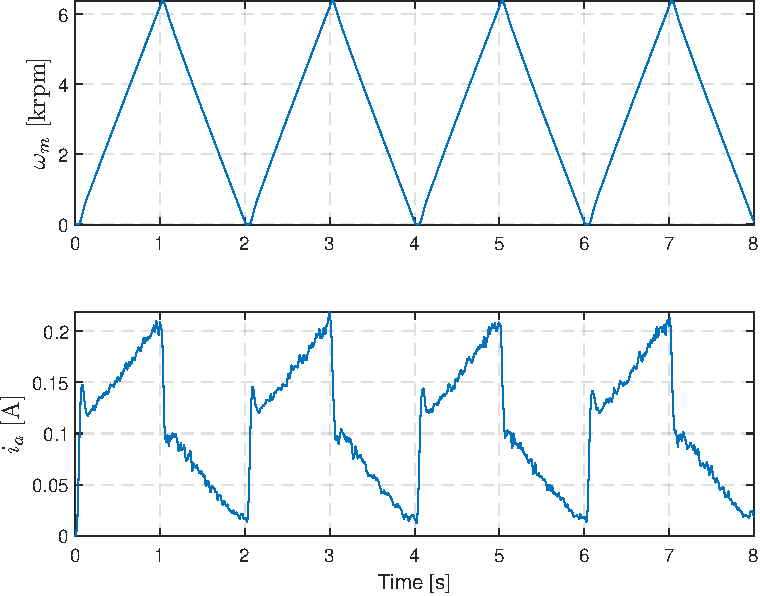
\includegraphics[scale=0.60]{images/Inertia_Estimate_ia_wm_Plot}}\quad
		\subfloat[]{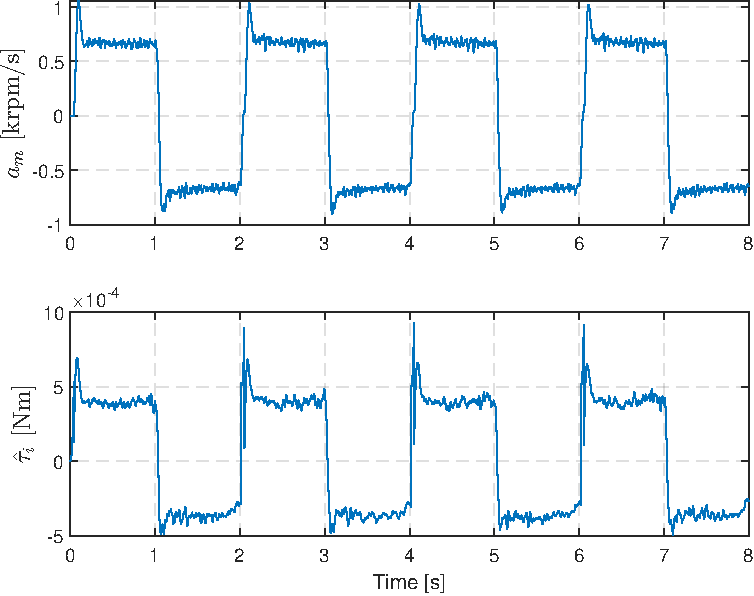
\includegraphics[scale=0.60]{images/Inertia_Estimate_taui_am_Plot}}
		\caption{Inertia estimation test: (a) speed and current profiles; (b) acceleration and inertial torque profiles.}
		\end{figure}
	

\end{document}

